\subsubsection{فرآیند پیش‌بینی خطا}
اکثریت پژوهش‌های پیش‌بینی خطا از روش‌های یادگیری ماشین  استفاده کرده‌اند. اولین گام در ساخت مدل پیش‌بینی تولید داده‌هایی با استفاده از آرشیو‌های نرم‌افزاری همچون سیستم‌های کنترل نسخه مانند گیت، سیستم‌های ردگیری مشکلات  مانند جیرا و آرشیو ایمیل‌ها است. هر یک از این داده‌ها بر اساس درشت دانگی پیش‌بینی می‌توانند نمایانگر یک سیستم، یک قطعه‌ی نرم‌افزاری\LTRfootnote{Component} (بسته\LTRfootnote{Package})، فایل کد منبع، کلاس و یا تابع باشد. یک داده حاوی چندین معیار (یا ویژگی) می‌باشد که از آرشیو‌های نرم‌افزاری استخراج شده و دارای برچسب "سالم" و "خطادار"  و یا تعداد خطاها است. پس از تولید داده‌ها با استفاده از معیارها و برچسب‌ها می‌توان به پیش پردازش داده‌ها پرداخت (مانند انتخاب معیار) که البته این امر اختیاری می‌باشد. پس از بدست آوردن مجموعه‌ی نهایی داده‌ها یک مدل پیش‌بینی را آموزش می‌دهیم که می‌تواند پیش‌بینی کند یک داده‌ی جدید حاوی خطا است یا خیر. تشخیص خطا خیز بودن داده\LTRfootnote{bug-proneness} معادل دسته بندی دودویی است و پیش‌بینی تعداد خطاها معادل رگرسیون می‌باشد. در شکل \ref{fig:prediction-process} فرآیند پیش‌بینی خطا نشان داده شده است. داده‌ها نمونه‌هایی هستند که می‌توانند خطادار  و بدون  خطا  بودن(   \lr{B = buggy} یا   \lr{C = clean} ) و یا تعداد خطا را نشان دهند. لازم به ذکر است که در یک مدل پیش‌بینی تنها از یک نوع از این داده‌ها استفاده می‌شود.

\begin{figure}[H]
	\centering
	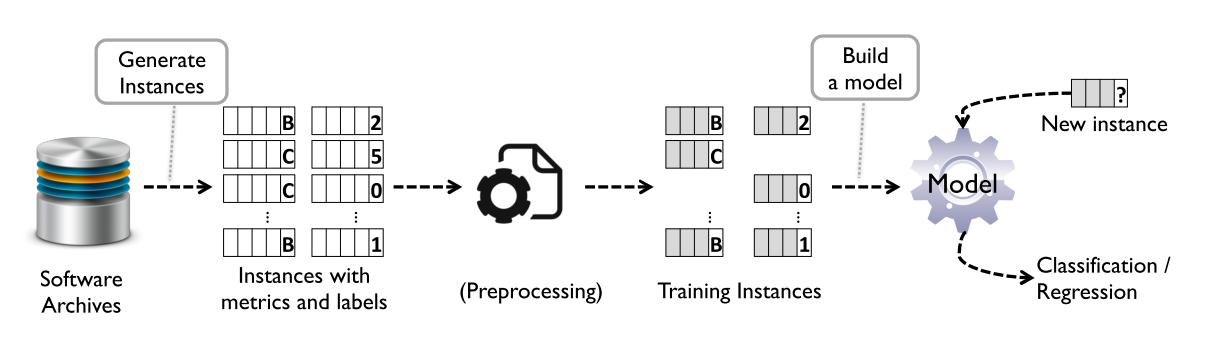
\includegraphics[width=1.0\textwidth]{images/prediction-process.PNG}
	 \caption{فرآینده پیش‌بینی نرم‌افزار \cite{nam2014survey}}
	\label{fig:prediction-process}
\end{figure}